% !TEX root = hazelnut-dynamics.tex

\begin{figure}[t]
\begin{subfigure}[t]{\textwidth}
\centering
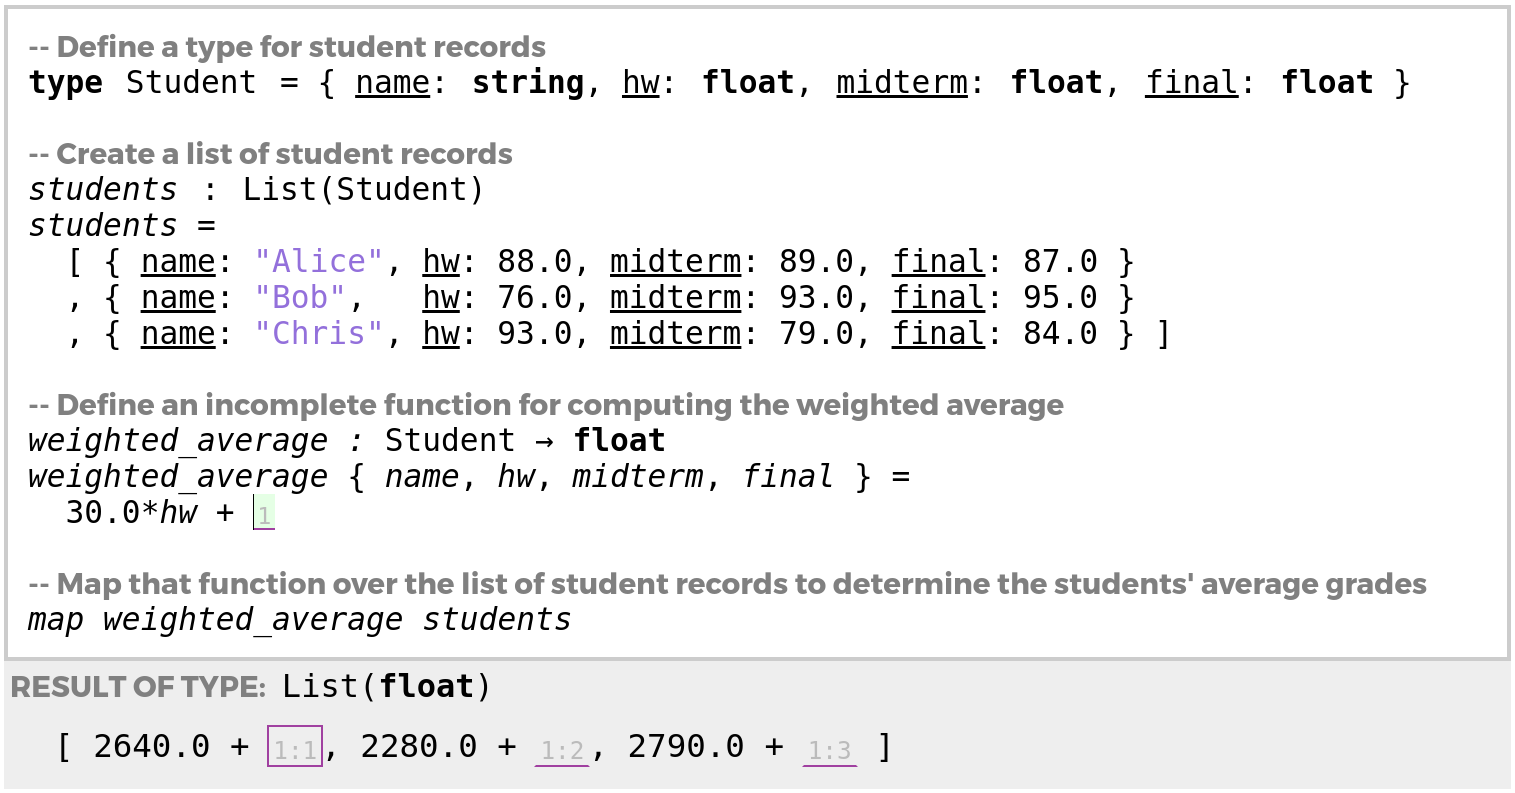
\includegraphics[width=\textwidth,interpolate=false]{images/grades-cell-mockup.png}
\vspace{-10px}
\caption{Evaluating an incomplete functional program past the first hole}
\label{fig:grades-cell-mockup}
\end{subfigure}

\vspace{10px}

\begin{subfigure}[t]{\textwidth}
\centering
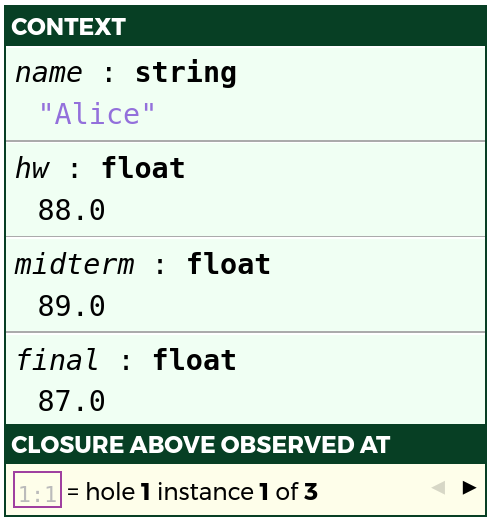
\includegraphics[width=0.31\textwidth,interpolate=false,valign=c]{images/grades-sidebar-1.png}
~${}^\blacktriangleright$
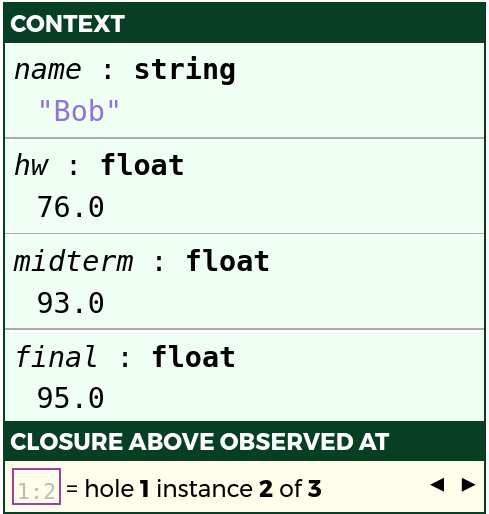
\includegraphics[width=0.31\textwidth,interpolate=false,valign=c]{images/grades-sidebar-2.png}
~${}^\blacktriangleright$
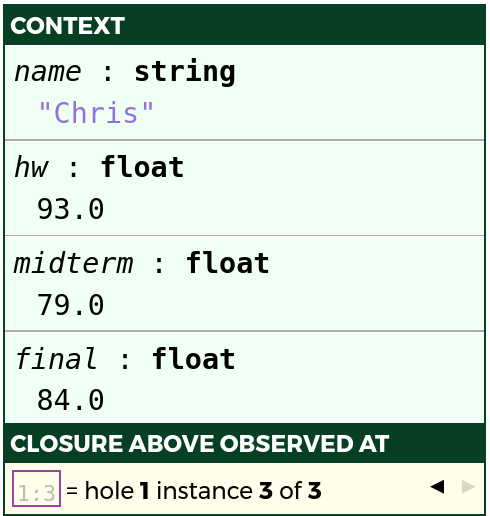
\includegraphics[width=0.31\textwidth,interpolate=false,valign=c]{images/grades-sidebar-3.png}
\caption{The live context inspector communicates relevant static \emph{and} dynamic information about variables in scope.}
\label{fig:grades-sidebar}
\end{subfigure}
% %% TODO once the code above is removed, scale up the screenshots
% 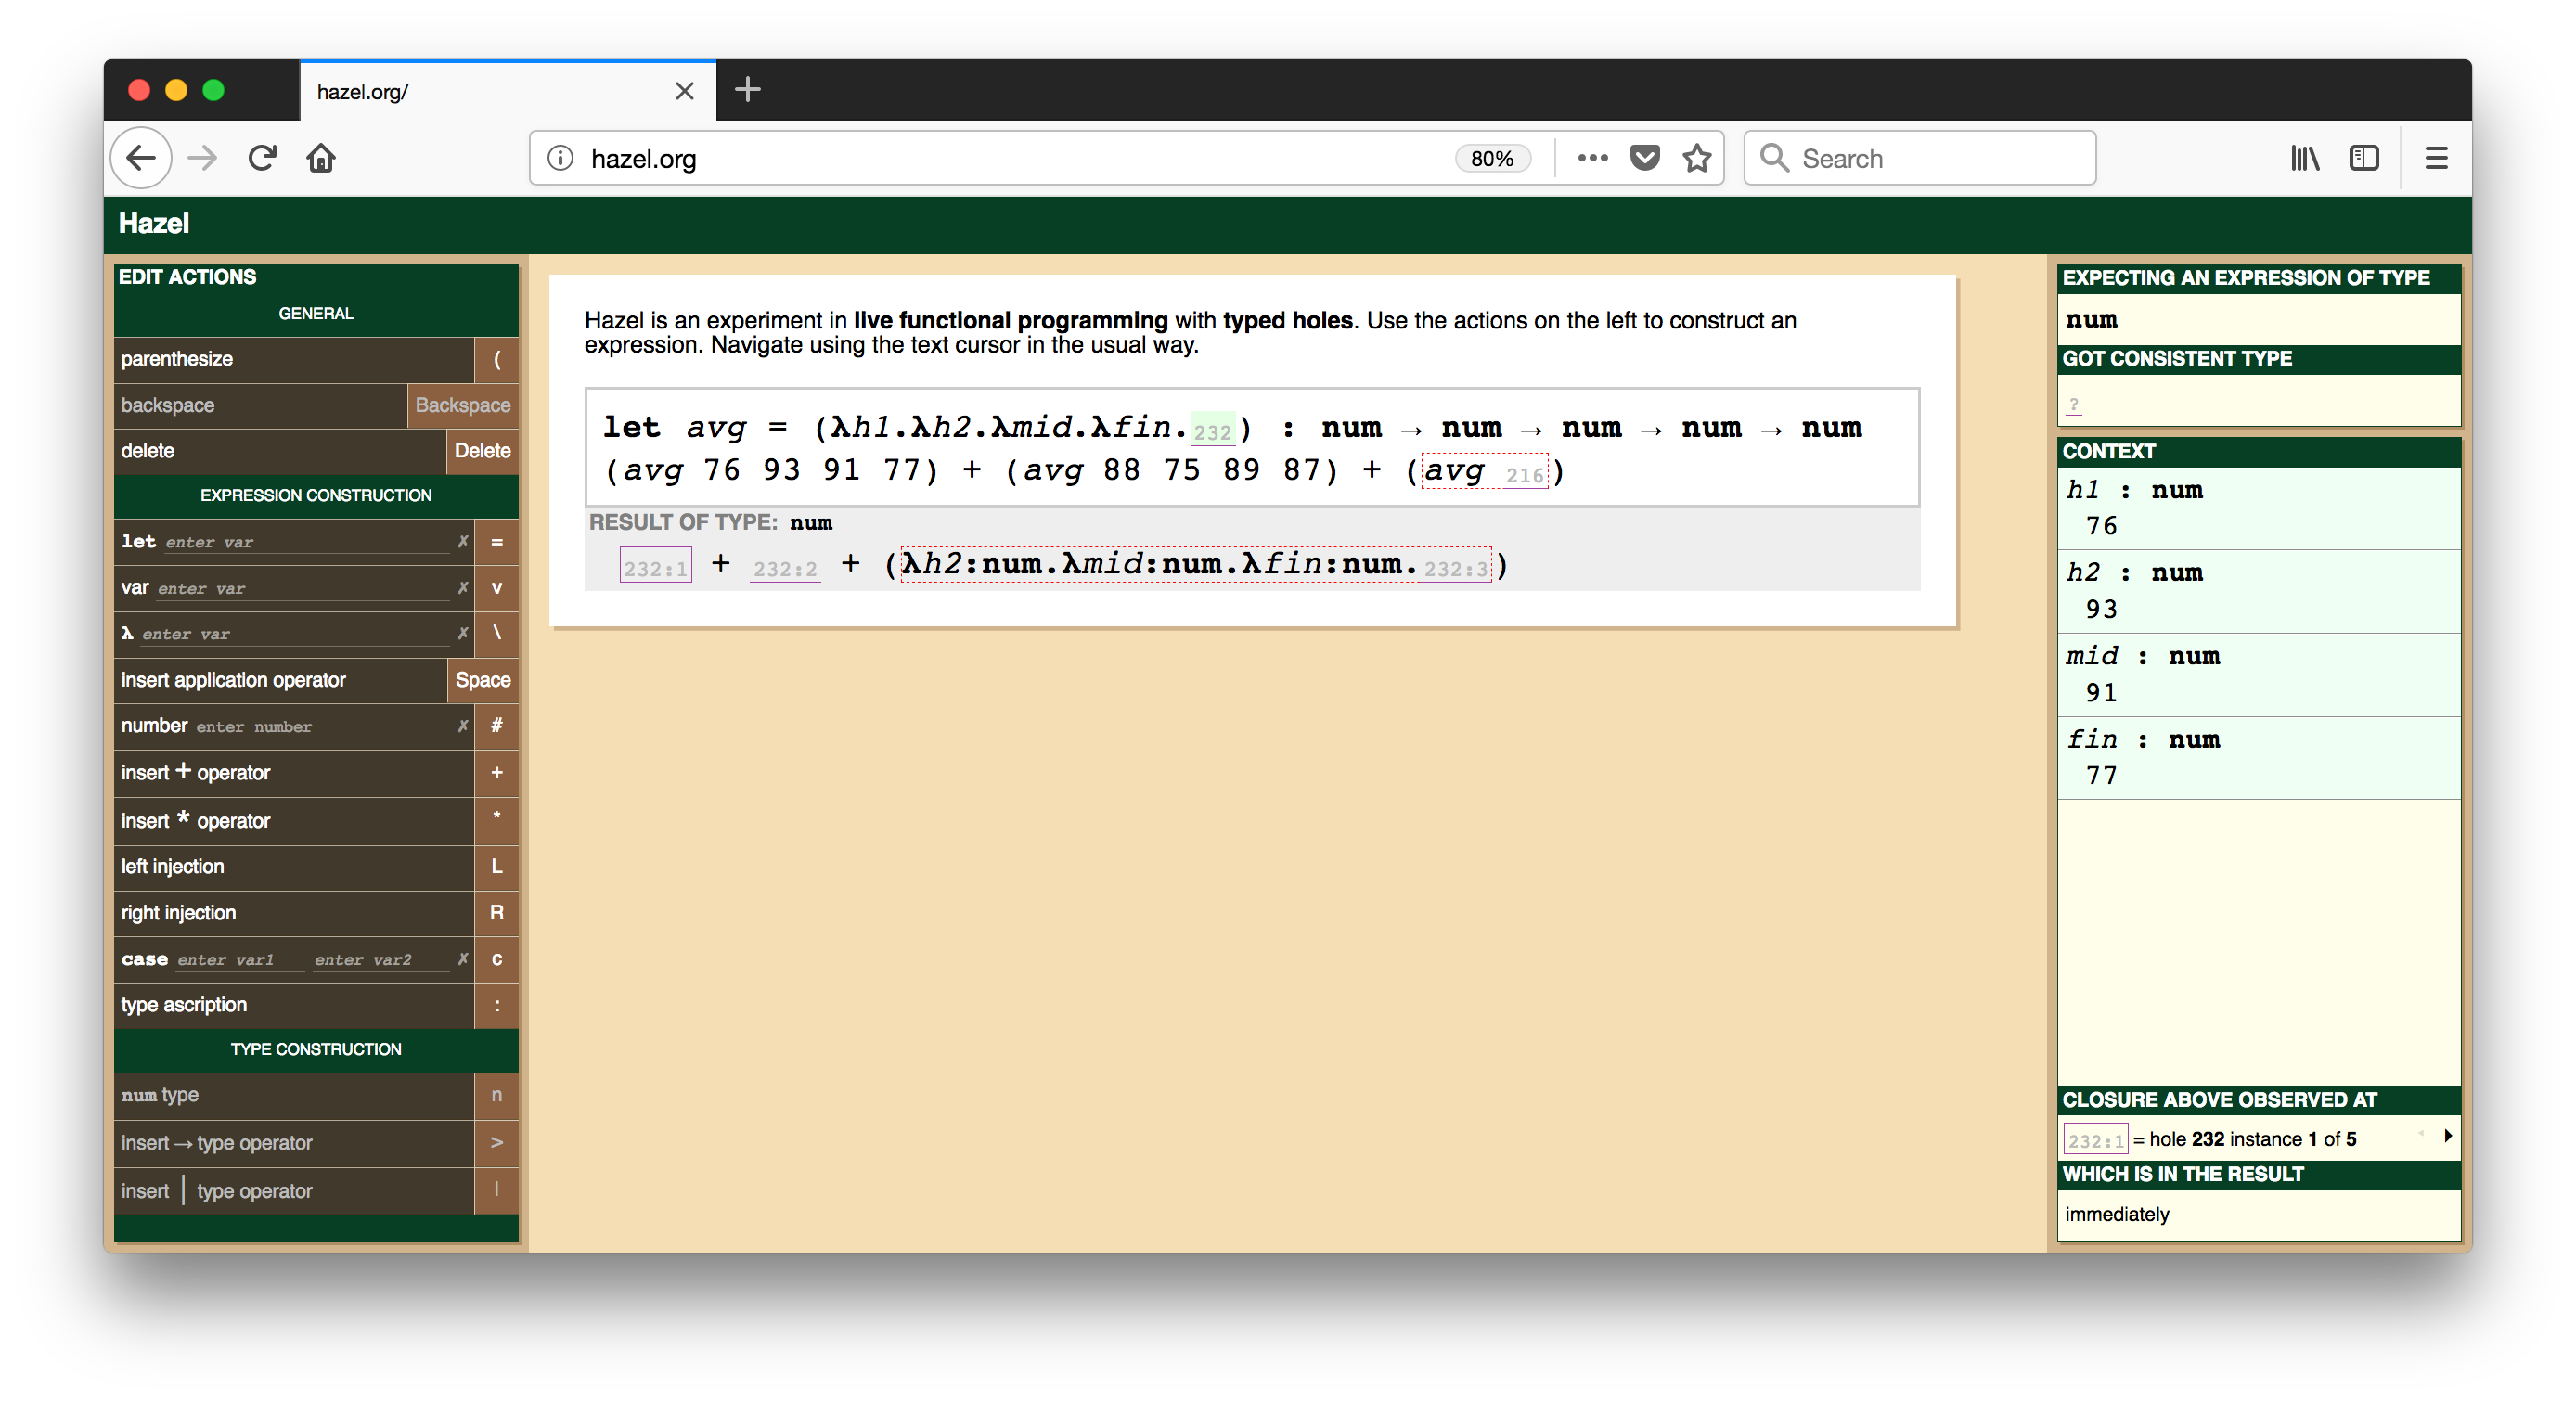
\includegraphics[scale=0.20]{images/hazel-placeholder-0.png}

% \rkc{Draw arrows and captions on the top figure to show how to get
% to the bottom figure.
% ser navigates to hole a, types + to create a plus, types * to create a
% multiplication, types \#10 to create 10, types vh1 to create variable use.}

% 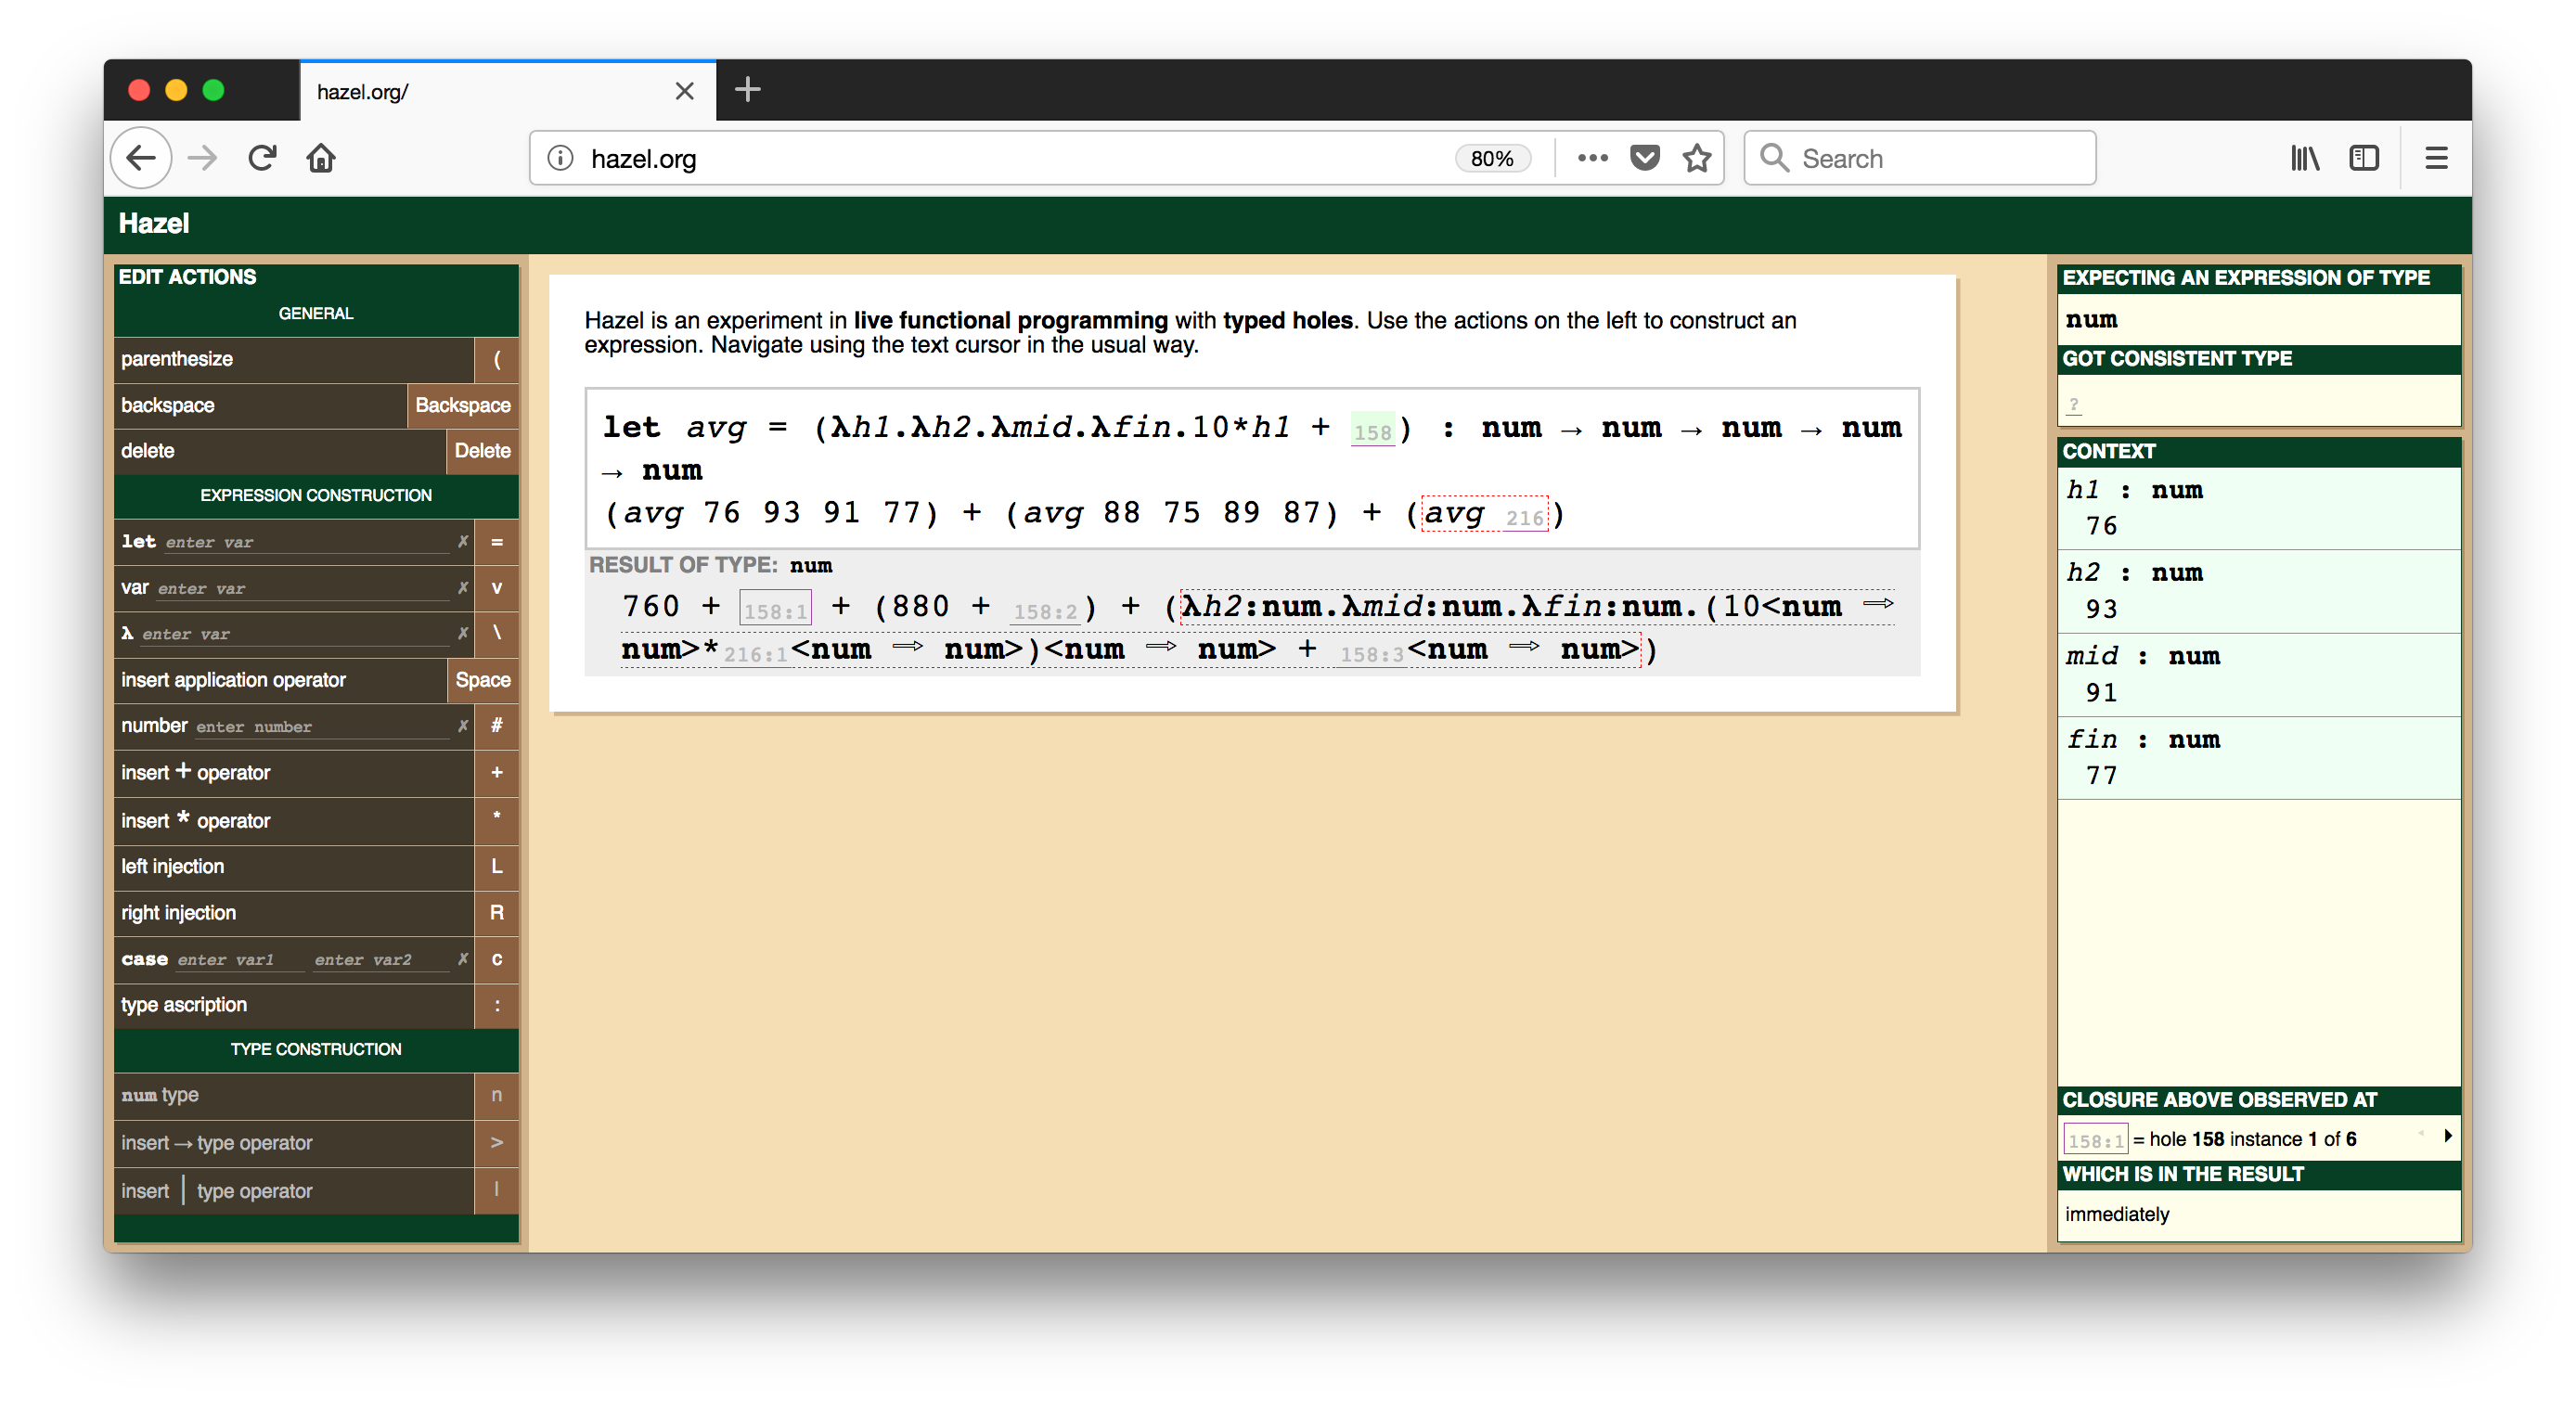
\includegraphics[scale=0.20]{images/hazel-placeholder-1a.png}
\vspace{3px}

\caption{Example 1: Grades}
\label{fig:grades-example}
\vspace{-5px}
\end{figure}
